\documentclass[a4paper,12pt]{article}

\usepackage[utf8]{inputenc}
\usepackage{listings}
\usepackage{graphicx}
\usepackage[margin=1in]{geometry}
\usepackage{listings}
\usepackage{float}
%\setlength{\parskip}{\baselineskip}

%opening
\title{Computer Vision - Virtual Whiteboard}
\author{Argentina Ortega Sáinz \and
        Nicolás Alfonso Laverde}   
\date{January 15, 2015}


\begin{document}
\pagenumbering{gobble}
\maketitle
\pagenumbering{arabic}
%---------------------------------------------------------------------------------------------%







\section[Introduction]{Introduction.\footnote{AOS}}
Tracking system for a predefined marker that can be used to paint as if it was a virtual whiteboard. The system would have the capabilities to recognize different coloured “virtual markers” (but one at a time), and to detect the strokes or traces made with them. Detected strokes are then draw.
The aim behind it is to be able to project the drawings (traces of the marker) into a screen using of a video projector, and even to the point of saving them. This will allow the digitalization of notes made by the user of the system (marker carrier), such as a teacher, for later distribution and inspection.
%---------------------------------------------------------------------------------------------%
\section[Objective]{Objective.\footnote{NLA}}
Design a vision system able to recognize the strokes made with a predefined marker in a flat surface and to transform the strokes into drawings for later projection.
\subsection{Specific Objectives}
\begin{itemize}
\item Design, calibrate and synchronize an orthogonal array of two cameras in order to capture videos simultaneously of a scene from different perspectives.
\item Process two videos from different perspectives in order to detect strokes performed by a pre-defined marker.
\item Simulate a whiteboard by drawing the detected strokes and later projecting the draws into a screen for visualization.
\end{itemize}
%---------------------------------------------------------------------------------------------%
\section[Motivation.]{Motivation.\footnote{AOS}}
Perception in a very important component of a autonomous system. Images and video signals provide a rich source of information about the environment in which an agent may be acting. Task like detection and recognition in scenes play a major part in most of the robotic applications, and so does it tracking. Applications where the agent must keep journal of the position of a moving object relay on speed and accuracy of the extraction of points in the space given images or video, which represents a position in a specific reference frame. Such systems deal with issues of calibration, synchronization and parallel processing in a efficient way, allowing a quick response according to the system design. Hence, with the virtual whiteboard we can deal with a tracking problem of a moving object in a semi-static scene, which can enlighten us in order to solve more complex task in the same field.
%---------------------------------------------------------------------------------------------%
\section[Description.]{Description.\footnote{NLA}}
The use of an orthogonal arrange of cameras allow us to reconstruct the 3D coordinates of the marker using 2D synchronized images, following a similar approach as mentioned in \cite{laganiere}. The board plane contains the "x" and "y" coordinates, which are obtained by the re-projection of points from the two views to the this plane. The "z" component (depth) will make two modes distinguishable: the “writing mode” and a “moving mode” . A similar approach is mentioned in \cite{zabulis}, but using hand gestures instead of markers.

\begin{figure}[H]
    \begin{center}
    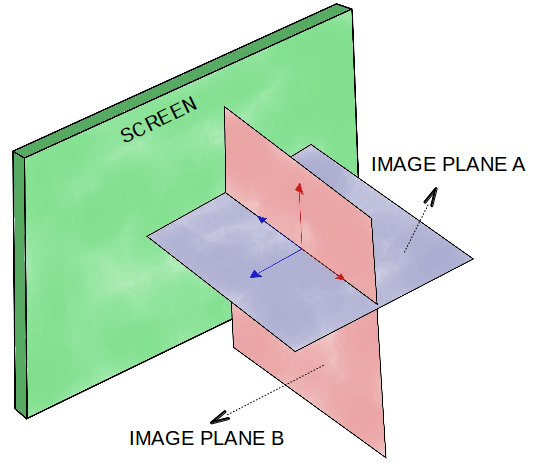
\includegraphics[width=8cm]{planesScheme.png}
    \caption{Planes Scheme.}
    The figure shows the three plains relevant to the system; the screen plane (in green) and  the two images planes (red and blue).
	\label{fig:planes}
    \end{center}
\end{figure}

The "writing mode" implies that the marker is close enough to the surface (screen) to enable the detection of the strokes, and therefore, drawing. The "moving mode" means that the marker can be moved, but the system will not detect the strokes of such movements, and therefore, no drawing is performed.

In other words, an "active drawing" volume is defined, which allow us to make the distinction between the modes. This active plane is parallel to the screen plane.

For the the system's output (drawing), we proposed to project from the back into the screen using a video-projector. Doing so, we could test the system at the same time; i.e. making the strokes and seeing the drawing correspondent to the movement of the marker. Projecting for the back allows us to avoid blocking the projected beam.

%------------------------------------------------------------------------------------------------%
\section[Set-Up.]{Set-Up.\footnote{AOS}}
The setup consists of two cameras; one camera is placed on the ceiling, over the board, and the other one is place in the side. Both cameras are to be mounted as close to the board as possible.

The selected cameras are two LiveCam from Microsoft, connected via USB. They have a frame rate of 30fps and a high resolution (up to 1920x1080). Additional, it offers an auto-focus feature from 0.1m to 10m. A halogen lamp was added as a result of non-uniform lighting in the room (as seen in the picture).

\begin{figure}[H]
    \begin{center}
	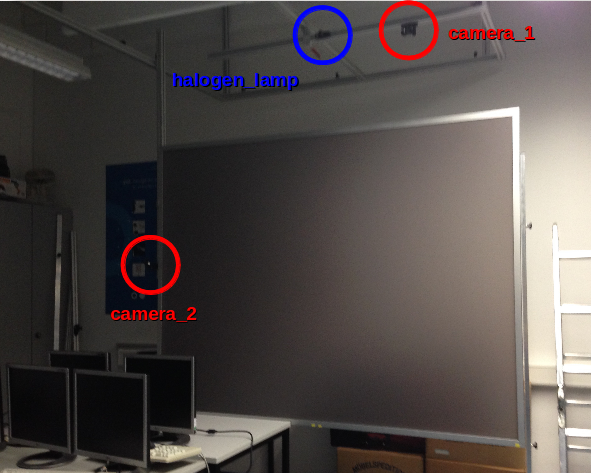
\includegraphics[width=12cm]{setupCams}
	\caption{Camera mounts and Light source positions.}
    The red circles indicate where the mounts for the cameras are. The blue circle indicates the position of the halogen lamp.
	\label{fig:setupcams}
    \end{center}
\end{figure}

\begin{figure}[H]
    \begin{center}
	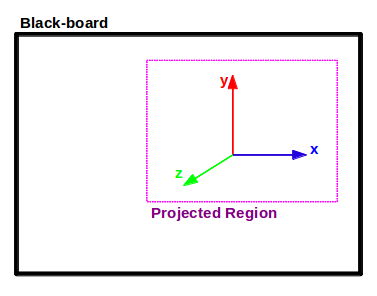
\includegraphics[width=8cm]{boardCoordinates}
	\caption{Board coordinate frame.}
    The purple dashed line corresponds to the effective area, where the video-beam will project the drawn strokes. This due to limitation in the distance between the video-beam and the physical screen
	\label{fig:board}
    \end{center}
\end{figure}

%---------------------------------------------------------------------------------------------%
\section[Data.]{Data.\footnote{AOS}}
As initialization a snapshot, one for each camera, is taken of the static background in order to be able to use them for segmentation later in the project. In addition, four snapshots are taken with the marker on each corner

Our data consists of snapshots of the two views taken by each camera respectively. The resolution of the images is 1920 x 1080 and a predefined number of frames was recorded while the strokes were being drawn. The frame rate is highly dependent of the laptop in which the cameras are connected; as consequence, the frame rate can not be fixed and is variable.

%---------------------------------------------------------------------------------------------%

\section[Approach]{Approach.\footnote{NLA}}
Our system proposal is comprised of two blocks: the marker detector block and the painter block. The maker detector is in charge of the detection of the marker in two synchronized views, and in the extraction of the pixel coordinates of the detected marker. Its inputs are two images from view 1 and 2, respectively, and it returns 2 pairs of pixel coordinates and a color. 

This is then fed to the painter block, which handles the re-projection of the coordinates from the two camera views into the plane of the virtual board. Therefore, its inputs are the output of the marker detector block and its output is the plot of such coordinates in the virtual board.

\begin{figure}[H]
    \begin{center}
	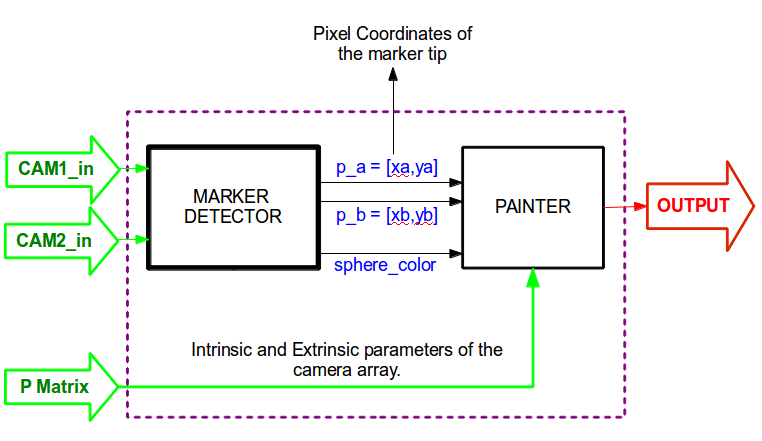
\includegraphics[width=8cm]{architecture}
	\caption{System Description.}
    Block-diagram of the virtual board system.
	\label{fig:descr}
    \end{center}
\end{figure}

Process-wise, we can identify 4 main stages: input, marker detection, position extraction and output. The flow of the system is serial, meaning that one stage is executed after the previous one has ended.
\subsection[Input Stage.]{Input Stage\footnote{AOS}}
Consist in the taking of the snapshot of the scene from the two cameras. This is in general terms our input data. At first, video capture was desired, but due to some hardware issues, the idea was dropped; instead, synchronously capture of images was implemented. Similarly, we wanted to design an online system, meaning that the processing of each pair of images is done parallel to the capture process, and so the output is seen in real time. At the end we opted for an offline version of the system; a session is recorded and then is processed, hence the output can't be seen in real time. 
This stage also deals with:
\begin{itemize}
        \item Control of the environment. We tried to control the lighting condition of our scene, but this prove to be a non-trivial task. The lighting conditions varied from session to session, which limited the performance of our system due to the design decision we made..
        \item Synchronization of the videos. This was done by syncing threads through the use of thread events. Each time the first thread is ready to take a snapshot it notifies the second one, and then both proceed to take a snapshot at approximately the same time.
        \item Calibration of the system. Every time a new session is recorded, a calibration routine must be followed. First, the system takes snapshots of the static background, which are later used in the maker detection stage. Second, the system captures 4 pairs of images where the user must be indicating where the corners of the virtual board are; this defines de region of interest and reduces the computational burden of the system in following stages. Lastly, some variables must be set, such as: paths and directories to read and write data, type of selection of the ROI (manual or auto), method of detection (color-threshold or background-segmentation) and the color of the marker (automatic detection of such feature was not implemented).
\end{itemize}

\subsection[Marker detection.]{Marker detection.\footnote{NLA}}
As mention before, two methods are implemented:

\subsubsection[Color-Threshold]{Color-Threshold\footnote{AOS}}
This was accomplished by using a selected Region of Interest, which had been converted to HSV color space. Previously selected lower and upper boundaries help us isolate the marker from the background. A median blur is applied. We use Otsu's binarization adaptive threshold to segment the marker from the scene, which calculates the threshold based on the histogram of the region of interest. This process is repeated for each frame, where only the region of interest is used during calculation in order to reduce the amount of data processed.

\subsubsection[Background-Segmentation.]{Background-Segmentation\footnote{NLA}}
This make use of the snapshot of the static background taken back in the input stage. First, we subtract the backgrounds from the current pair of frames, respectively. Then, a binary adaptive thresholding is applied, to delete noise pixels and regions in the frames which were are in principle the same, but due to the lighting conditions seem like a new object was introduced to the scene. This allow us to isolate the marker and the user. 

Applying a crop in the frame using the coordinates of the previously computed ROI, the isolation of the marker is further enhanced. Finally, contours are found, and the bigger one is selected, which then is used to compute the minimal circle that encloses the contour. This circles is said to be the marker.


\begin{figure}[H]
    \begin{center}
	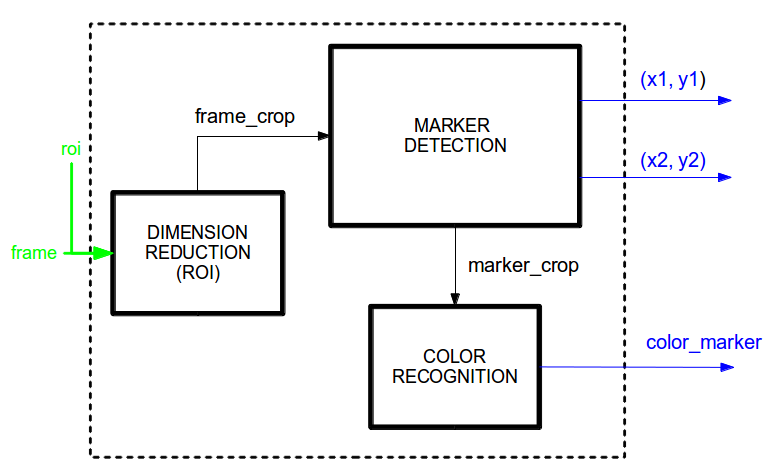
\includegraphics[width=8cm]{marker-stage.png}
	\caption{System Description.}
    Block-diagram of the marker detector stage.
	\label{fig:mark}
    \end{center}
\end{figure}

\subsubsection[Color recognition]{Color recognition.\footnote{AOS}}
It was implemented but discarded due to the high dependency with the lighting conditions. The way it was implemented was by analysis histograms computation of a isolated marker (an image were only the marker is presented). The color was detected in the RGB color space by using the RGB values found at the center of the circle that encloses the marker at the corner configuration sequence. HSV histogram computation was also implemented, fitting a Gaussian distribution among the three components of the histogram for later calculations of probabilities of a pixel to belong to a certain color.

\subsection[Position reconstruction.]{Position reconstruction.\footnote{NLA}} 
Once we have the marker detected in each frame, the next step is to get the world coordinates back from the image coordinates. We tried diverse method for calibration of two cameras, from stereo calibration, multiple-view geometry theory, fundamental matrix correspondence and homography computations. At the end, we decided to compute a homography using the y-pixel coordinate from view 1 (side view) and the x-pixel coordinate from view 2 (top view), and the homography between this set of points to the virtual board was calculated. 

The corner snapshots used for the automatic ROI extraction were used, given that there are four corners which correspond to the boundaries of the board. The homography was extracted and then used for re-projection of the marker position in the 2 views to the virtual board.

\begin{center}
$ [x_{board}, y_{board}]_{pixel}= H*[x_{view2}, y_{view1}]_{pixel} $
\end{center}


\subsection[Output Stage]{Output Stage\footnote{NLA}} 
The stroke vector obtained from the position reconstruction is used to draw the points (positions) back into the screen. The points are drawn according to the color selected and projected to the glass screen using a video-projector from the back.

%---------------------------------------------------------------------------------------------%
\subsection[Results]{Results}

\begin{itemize}
\item Snapshots captured synchronized from both cameras. \footnote{AOS}
\begin{figure}[H]
    \begin{center}
	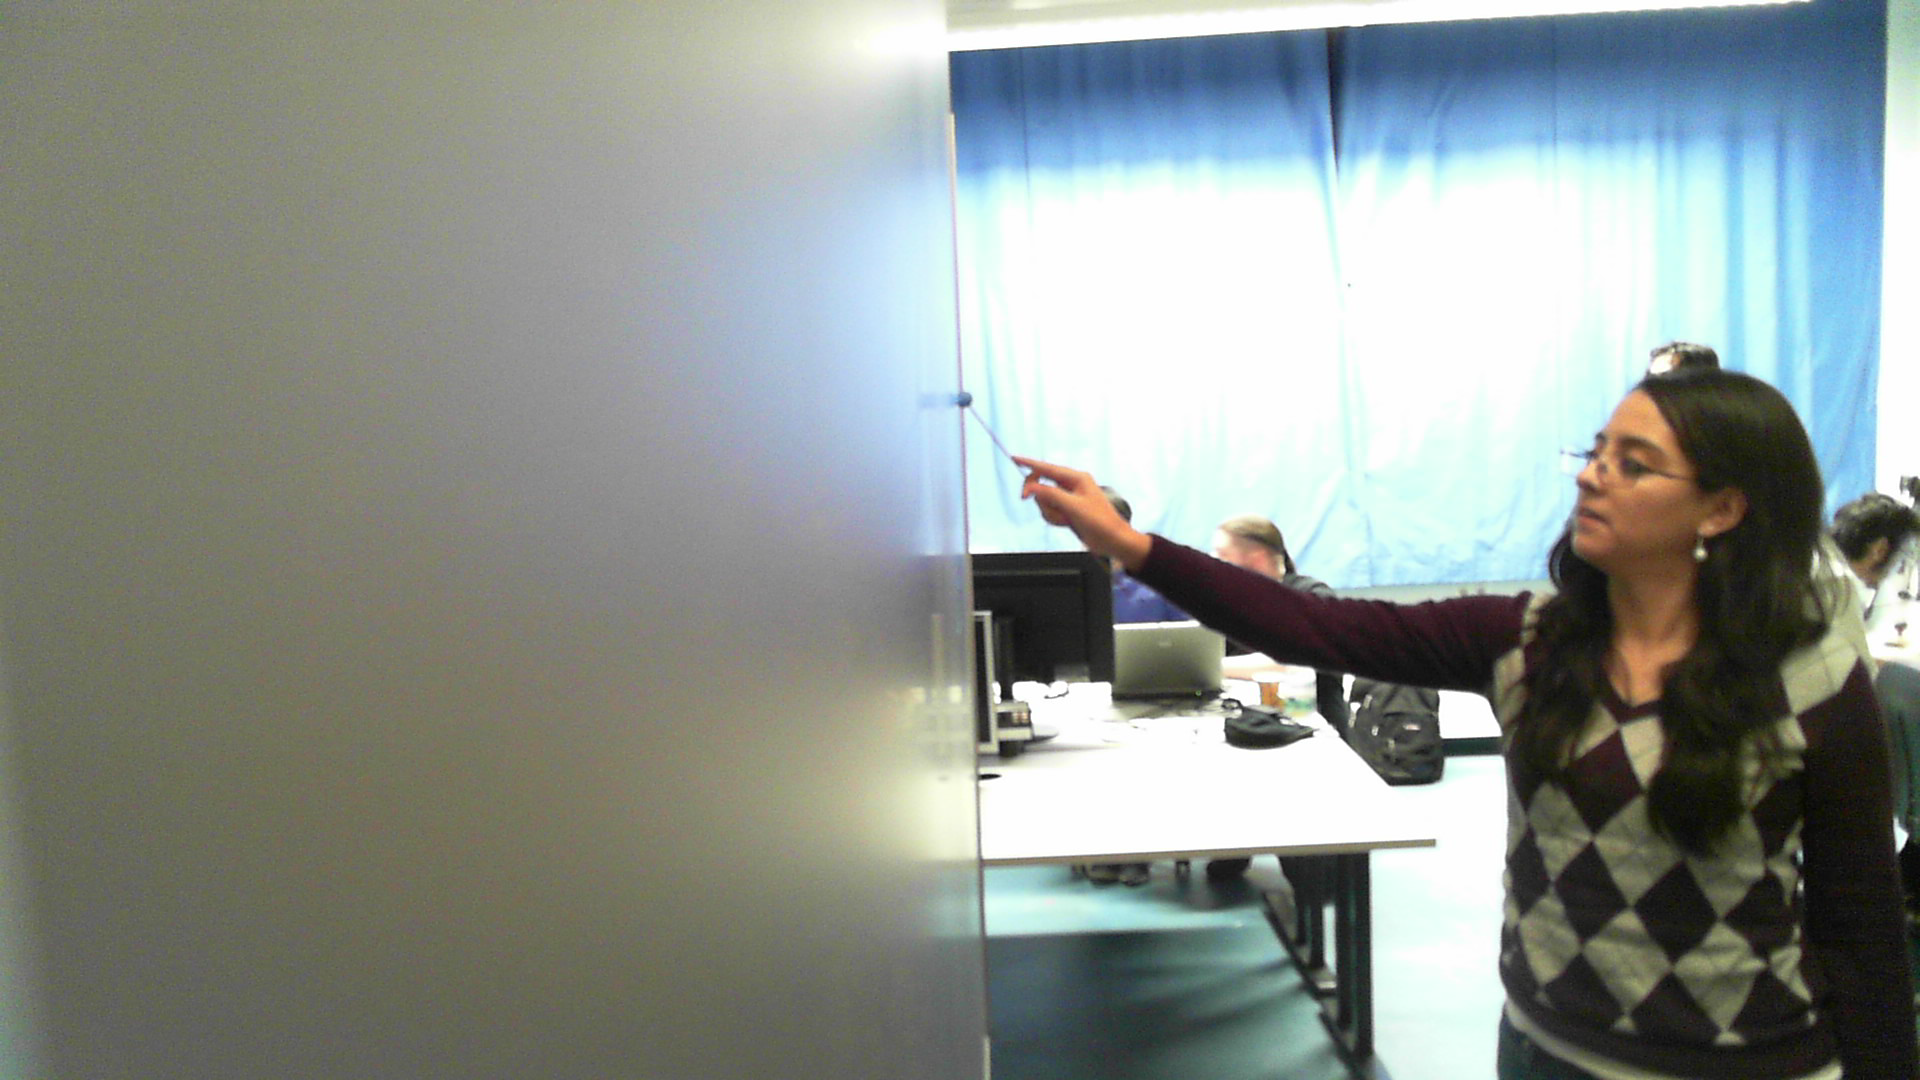
\includegraphics[width=0.45\textwidth]{FrameSide}
	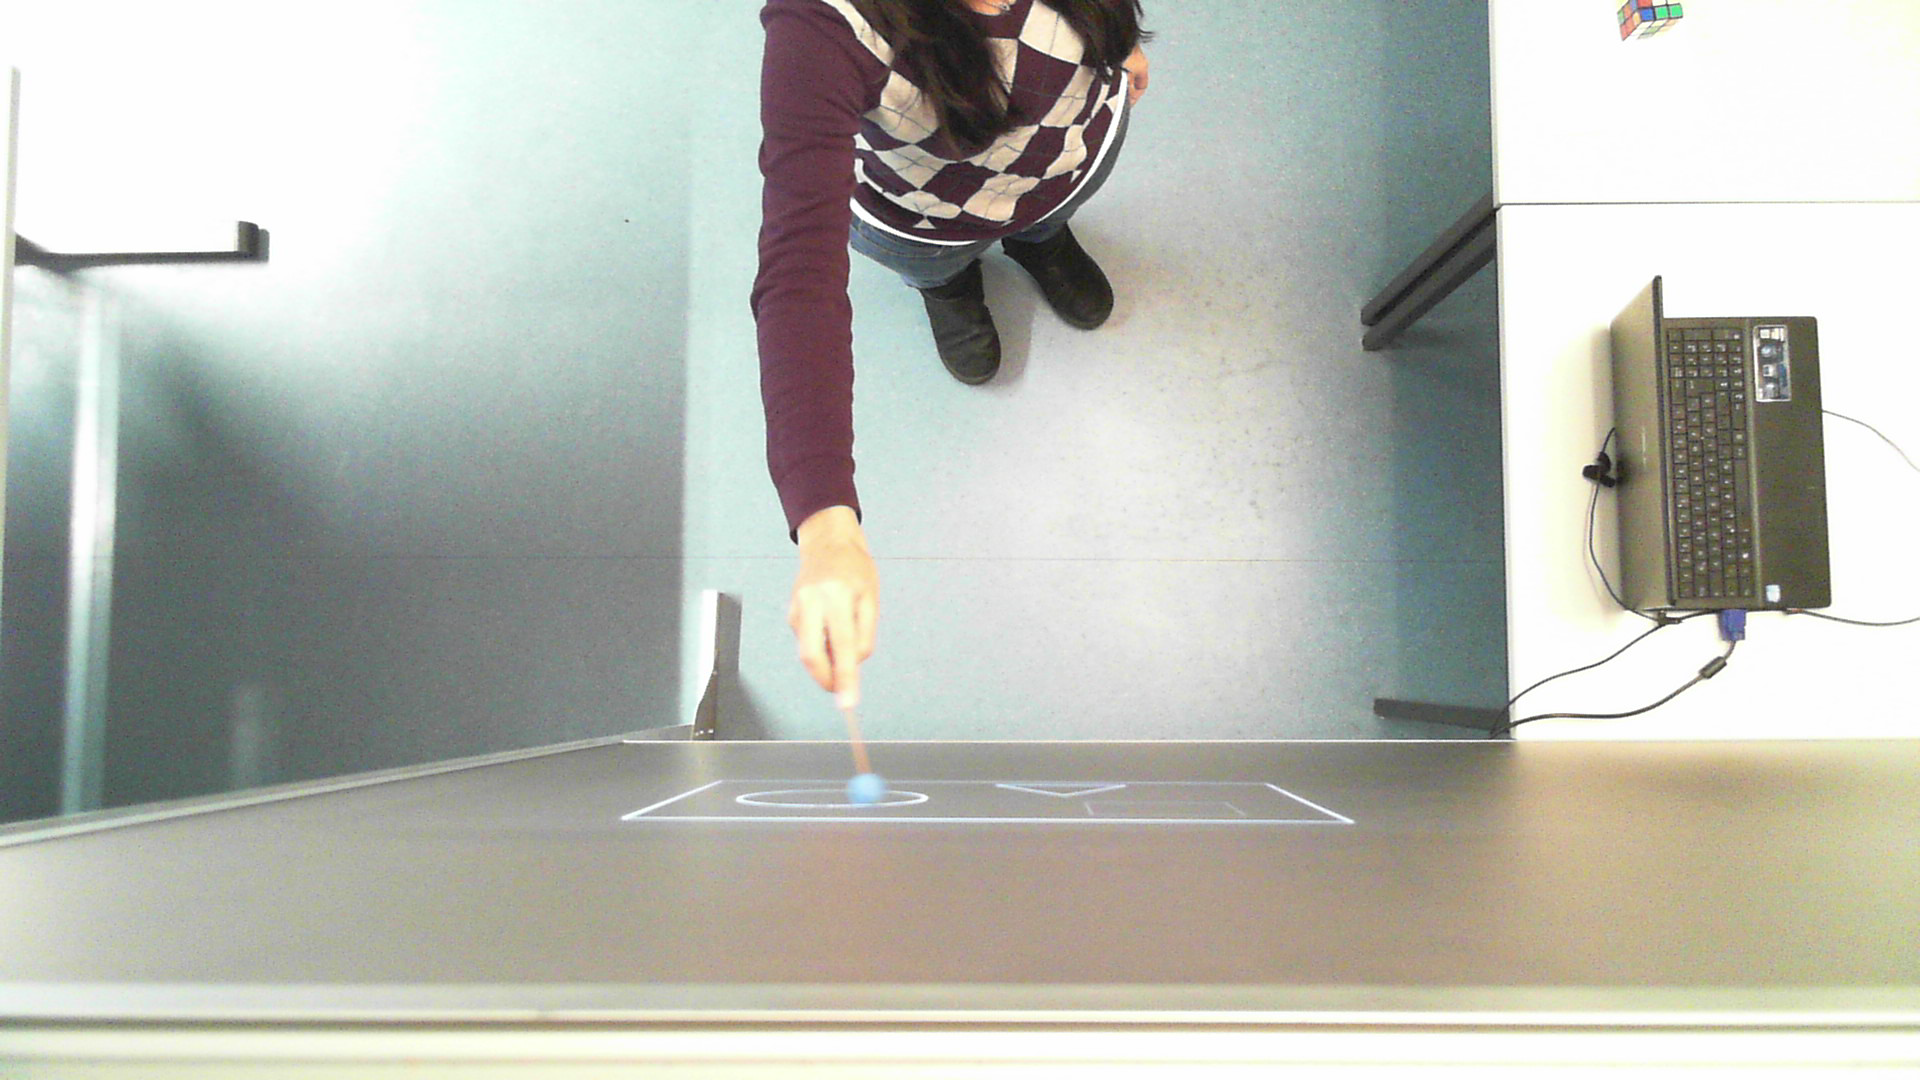
\includegraphics[width=0.45\textwidth]{FrameUp}
	\caption{Two snapshots taken simultaneously.}

	\label{fig:video}
    \end{center}
\end{figure}
\newpage
\item Identification of at least 3 colors to be used on three different markers.\footnote{AOS}
\begin{figure}[H]
    \begin{center}
	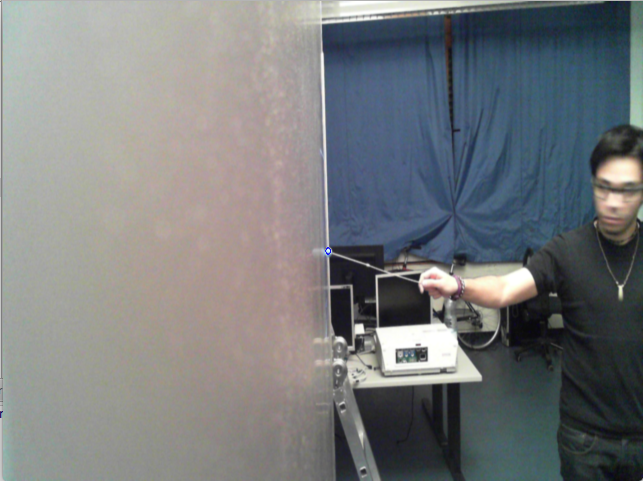
\includegraphics[width=0.45\textwidth]{MarkerSide}
	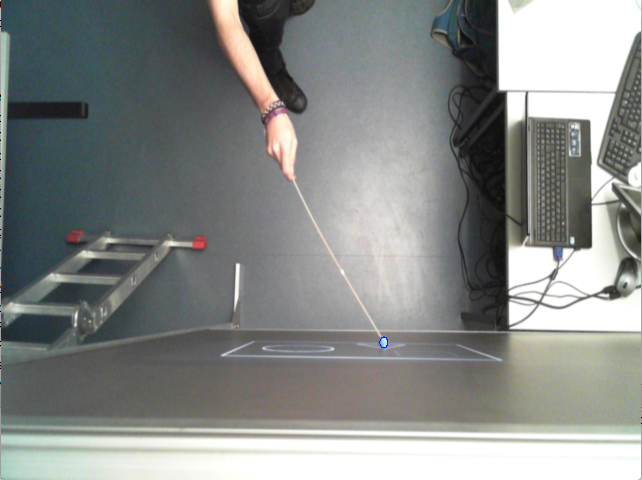
\includegraphics[width=0.45\textwidth]{MarkerUp}
	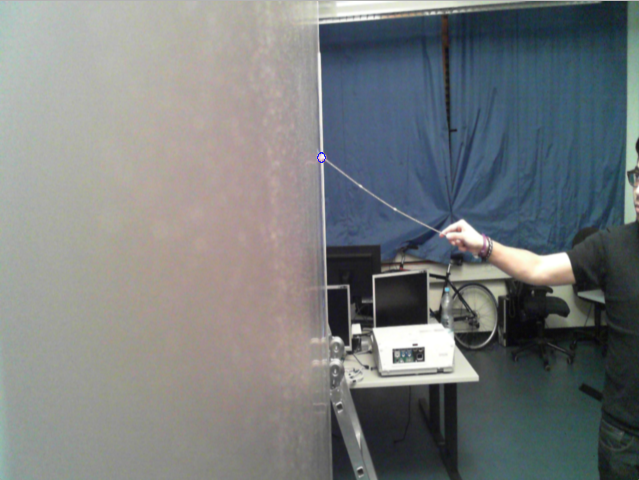
\includegraphics[width=0.45\textwidth]{RedSide}
	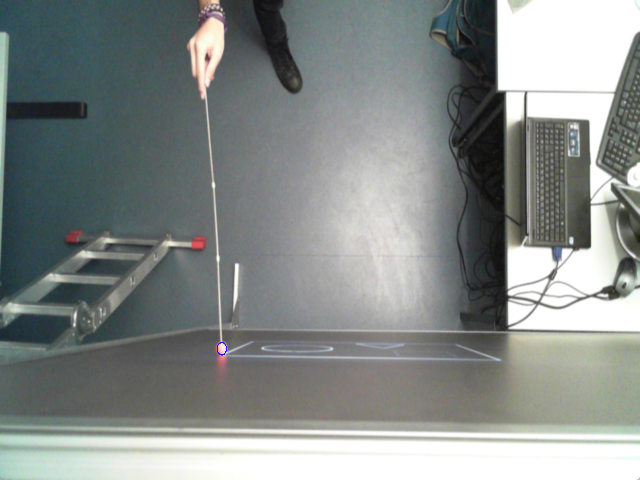
\includegraphics[width=0.45\textwidth]{RedUp}
	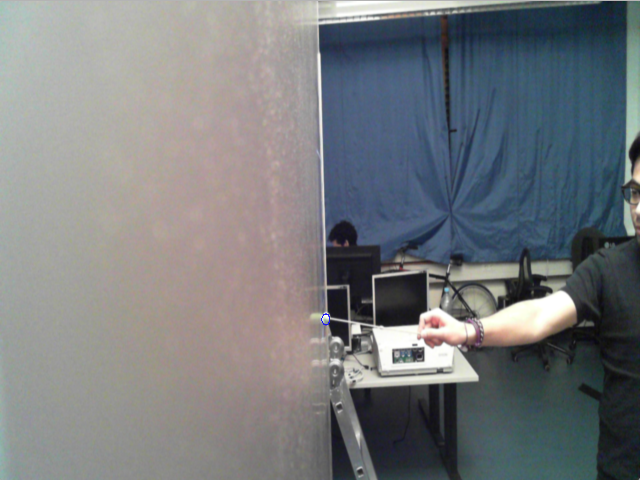
\includegraphics[width=0.45\textwidth]{GreenSide}
	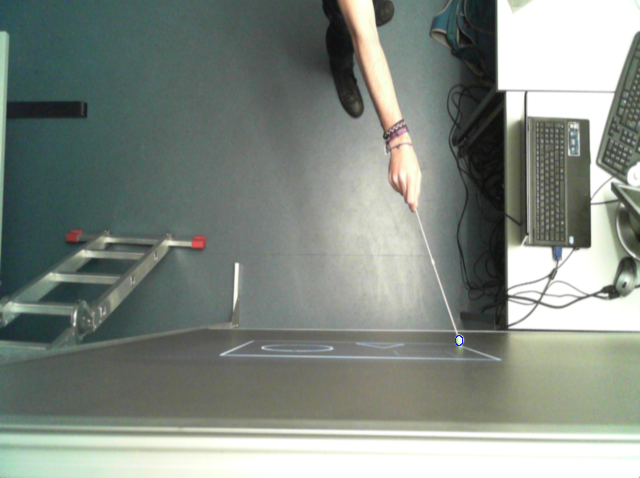
\includegraphics[width=0.45\textwidth]{GreenUp}
	\caption{Marker detection}
    Marker detected in both views. This is then used to detect the color of the stroke.
	\label{fig:marker}
    \end{center}
\end{figure}
\newpage
\item Guideline\footnote{NLA}
\begin{figure}[H]
	\begin{center}
	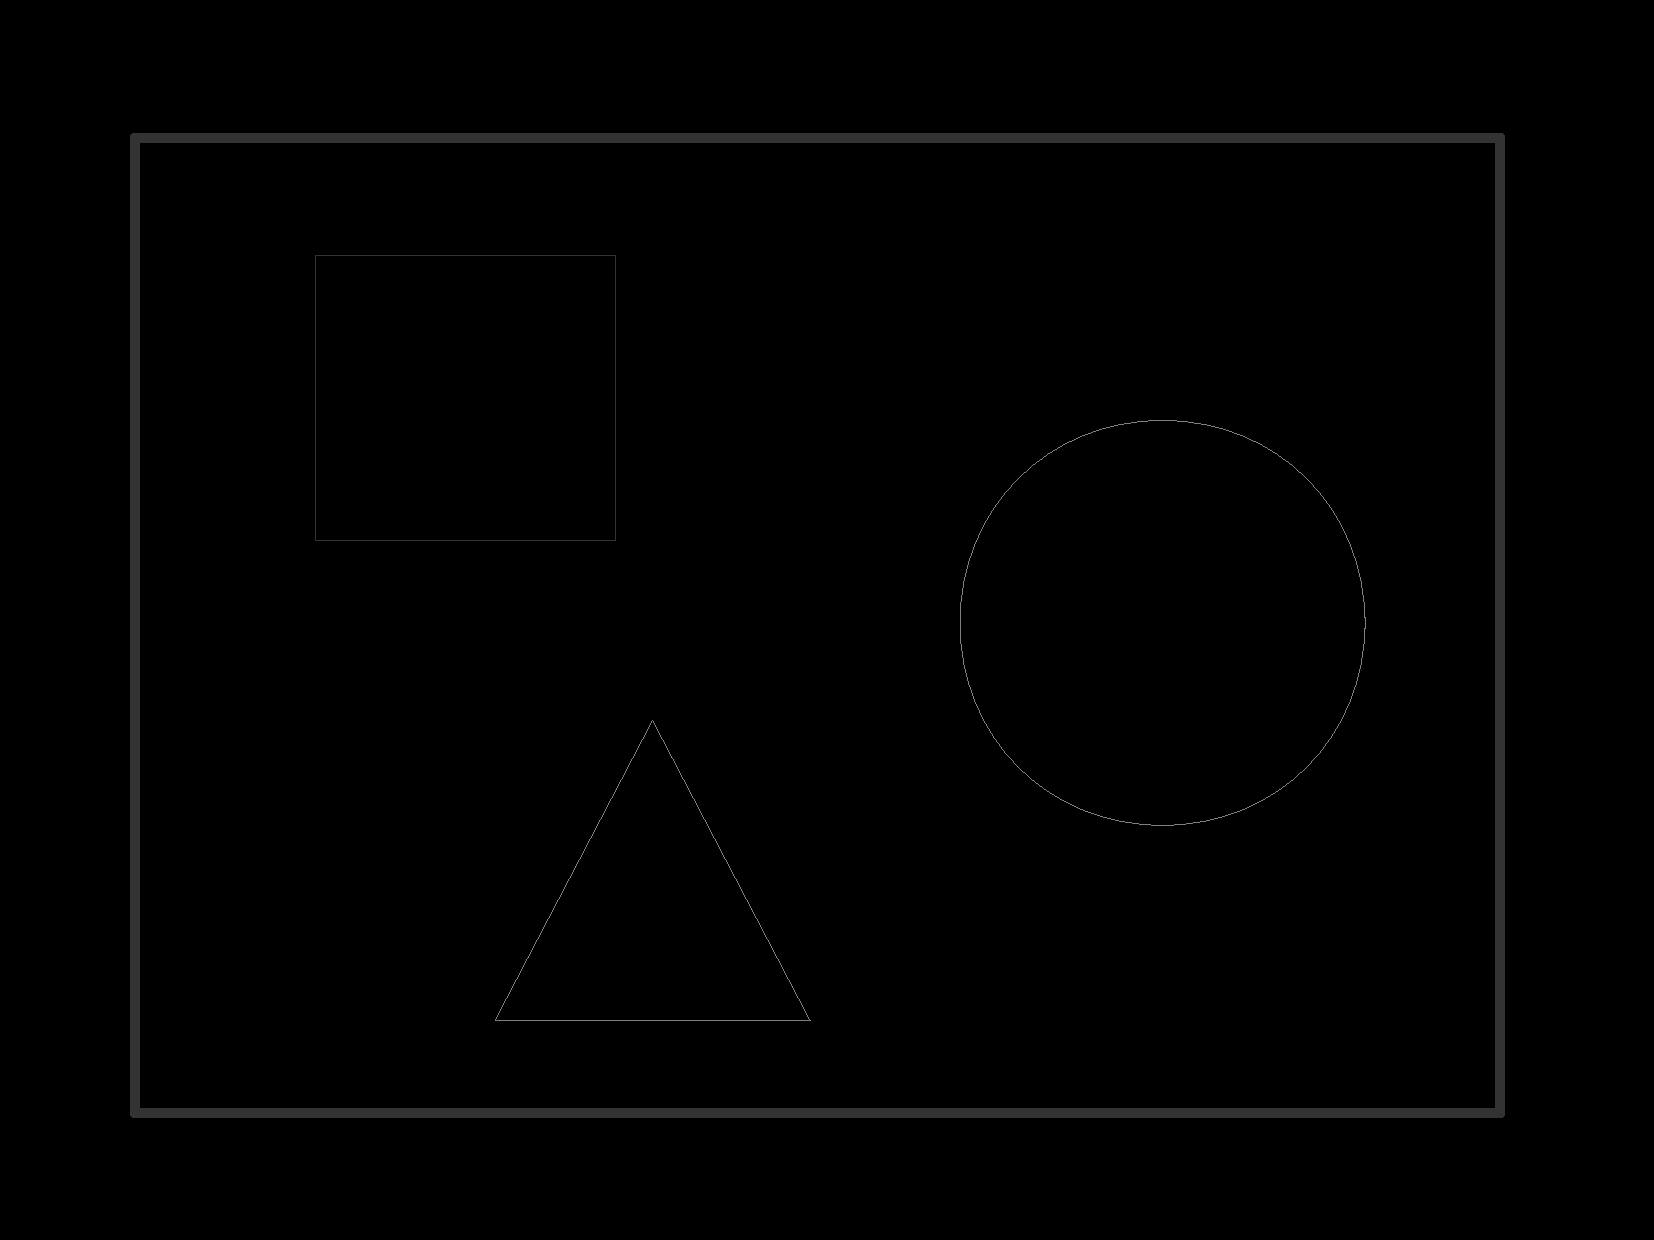
\includegraphics[width=0.45\textwidth]{guideline}
	\caption{Raw shapes used as guideline for testing purposes. Each session, the user tried to follow the contour of the shapes as close as possible.}
	\label{guide}
	\end{center}
\end{figure}
\newpage
\item Output of the system\footnote{NLA}
\begin{figure}[H]
\begin{center}
	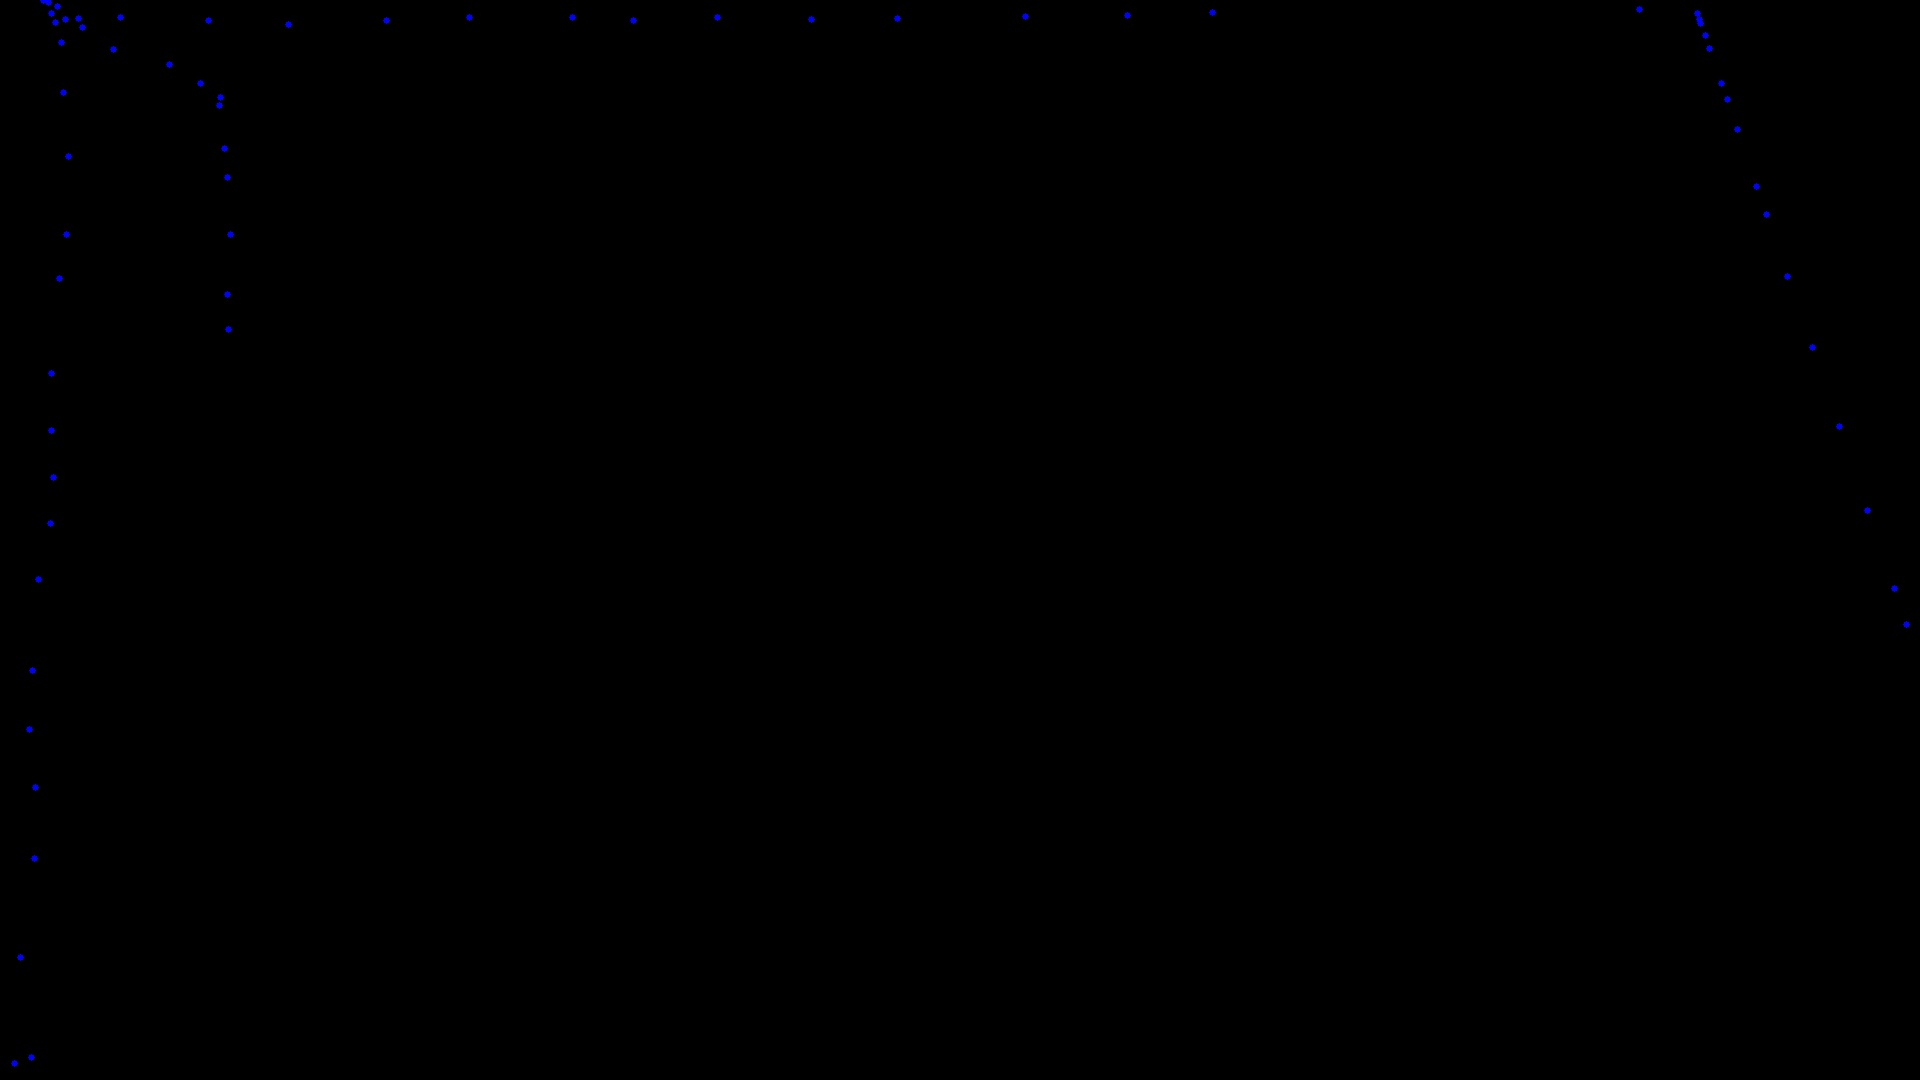
\includegraphics[width=6 cm]{result3_board.jpg}
	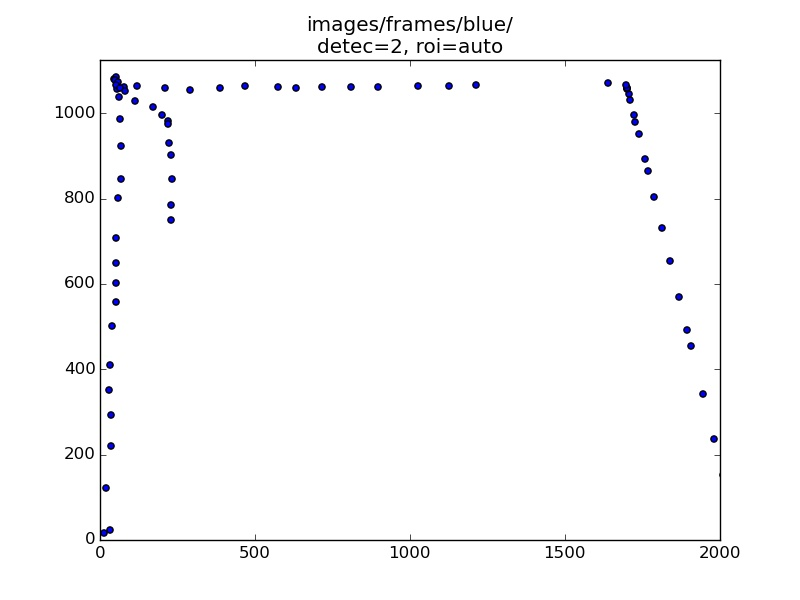
\includegraphics[width=6 cm]{result3_plot.jpg}\\
	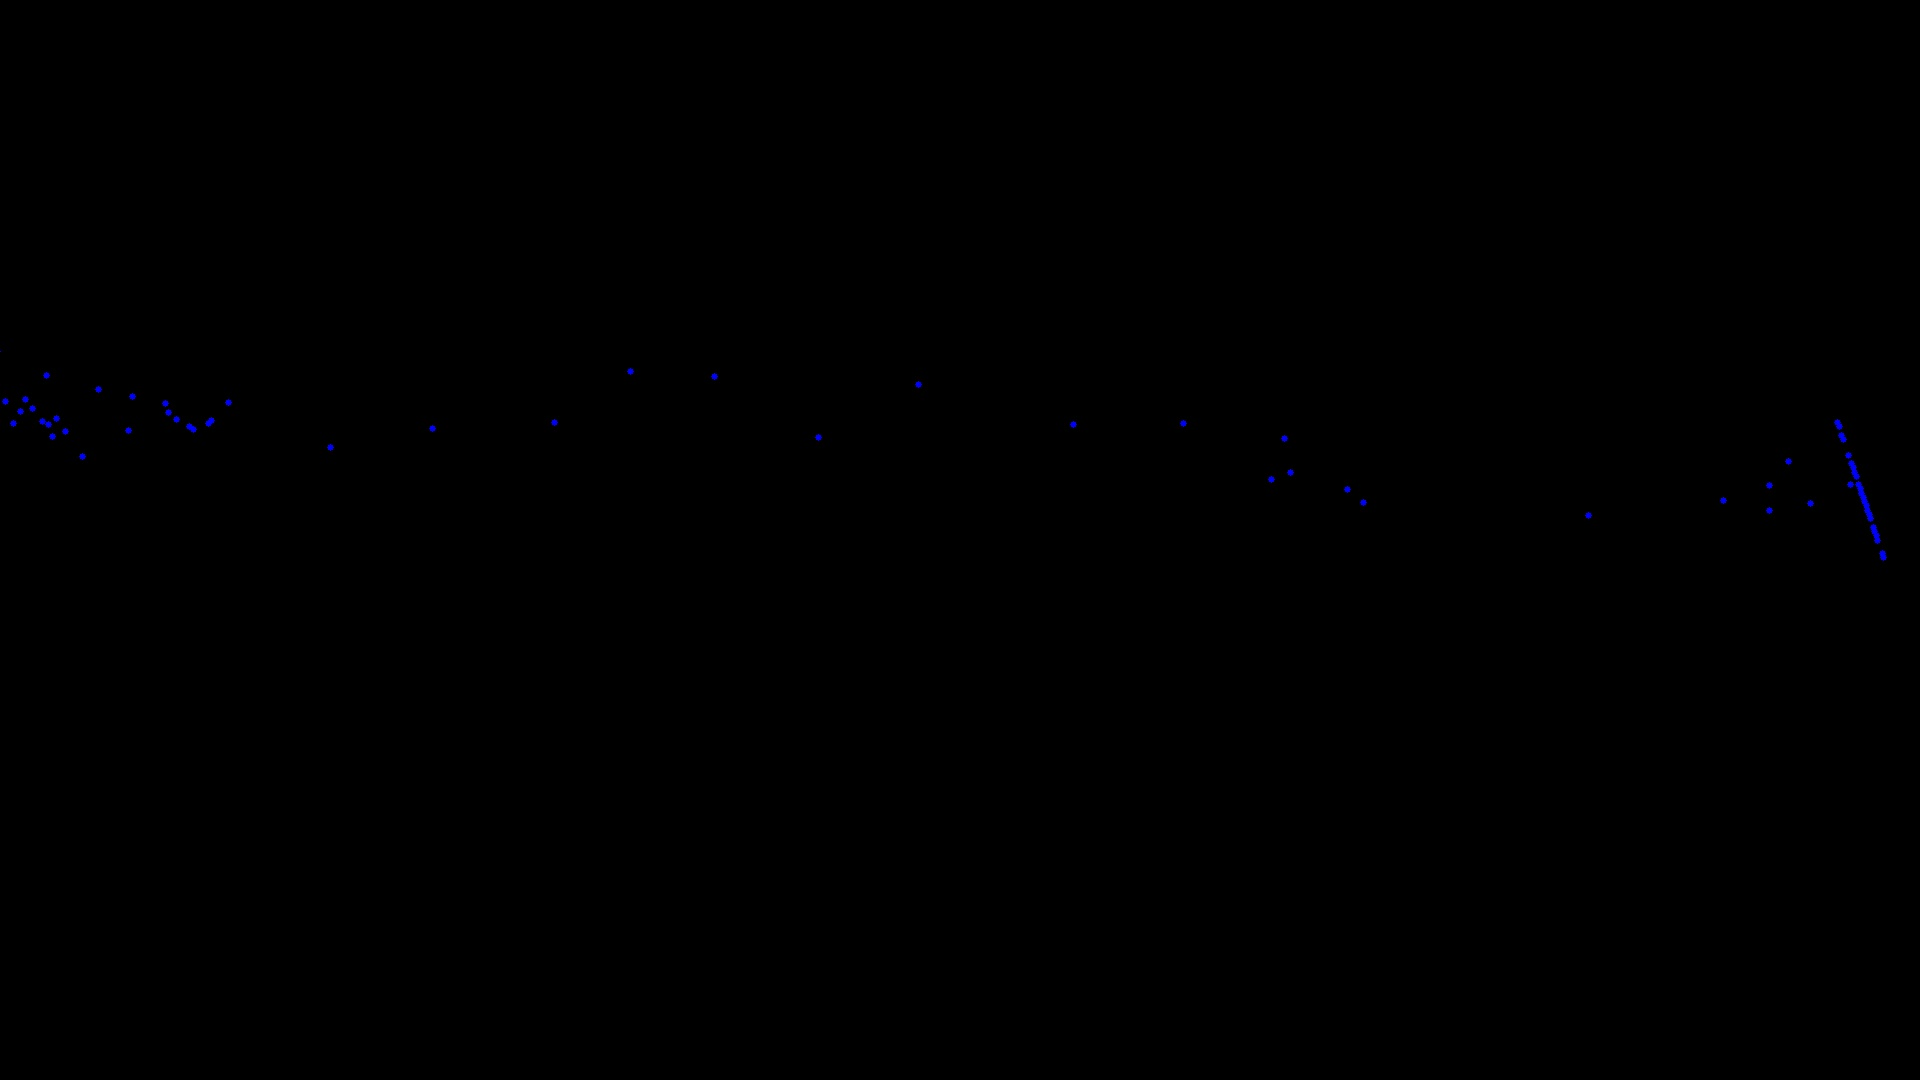
\includegraphics[width=6 cm]{result1_board.jpg}
	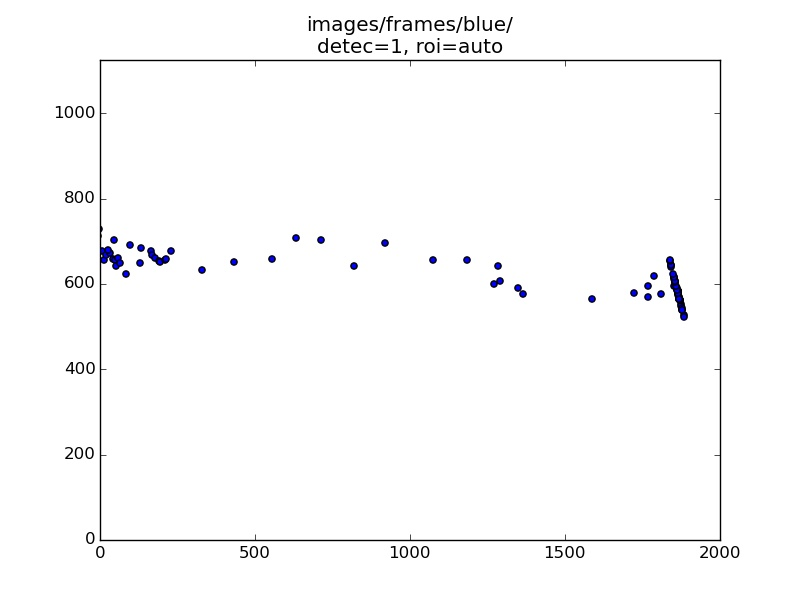
\includegraphics[width=6 cm]{result1_plot.jpg}\\
	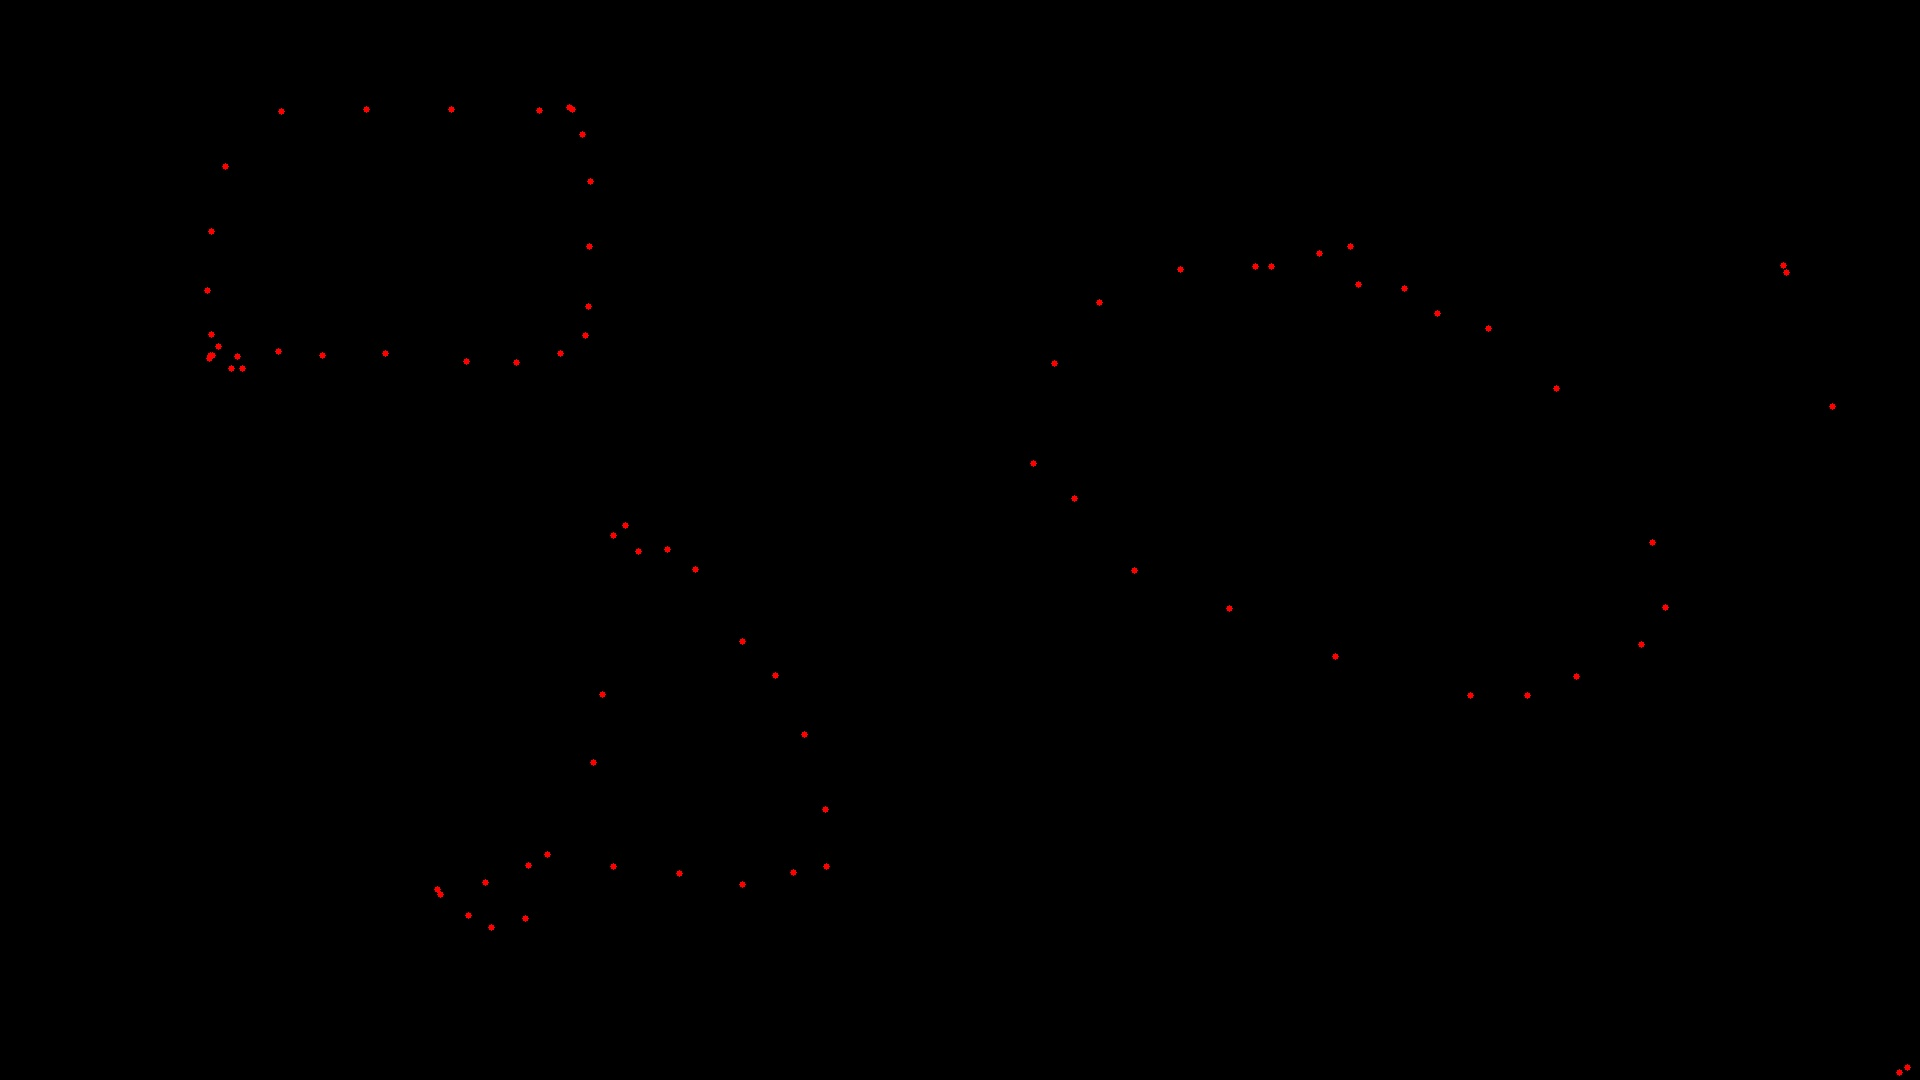
\includegraphics[width=6 cm]{result4_board.jpg}
	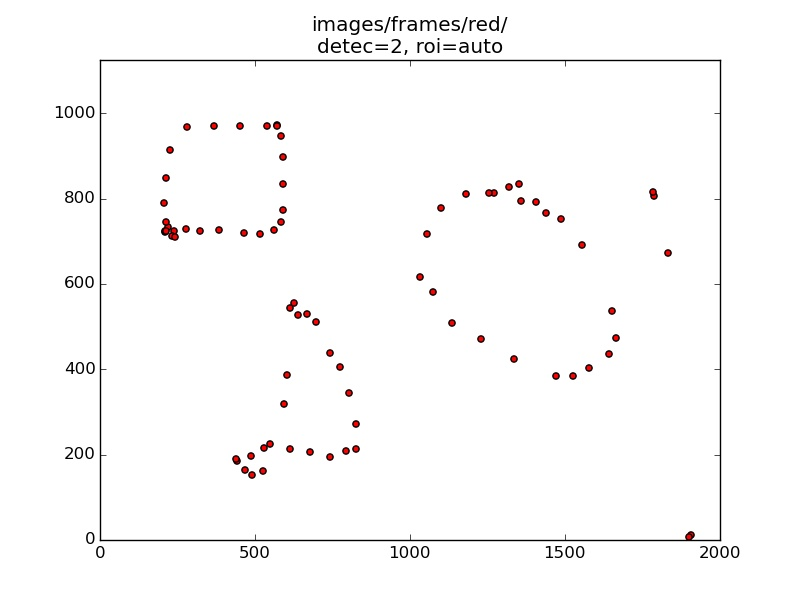
\includegraphics[width=6 cm]{result4_plot.jpg}\\
	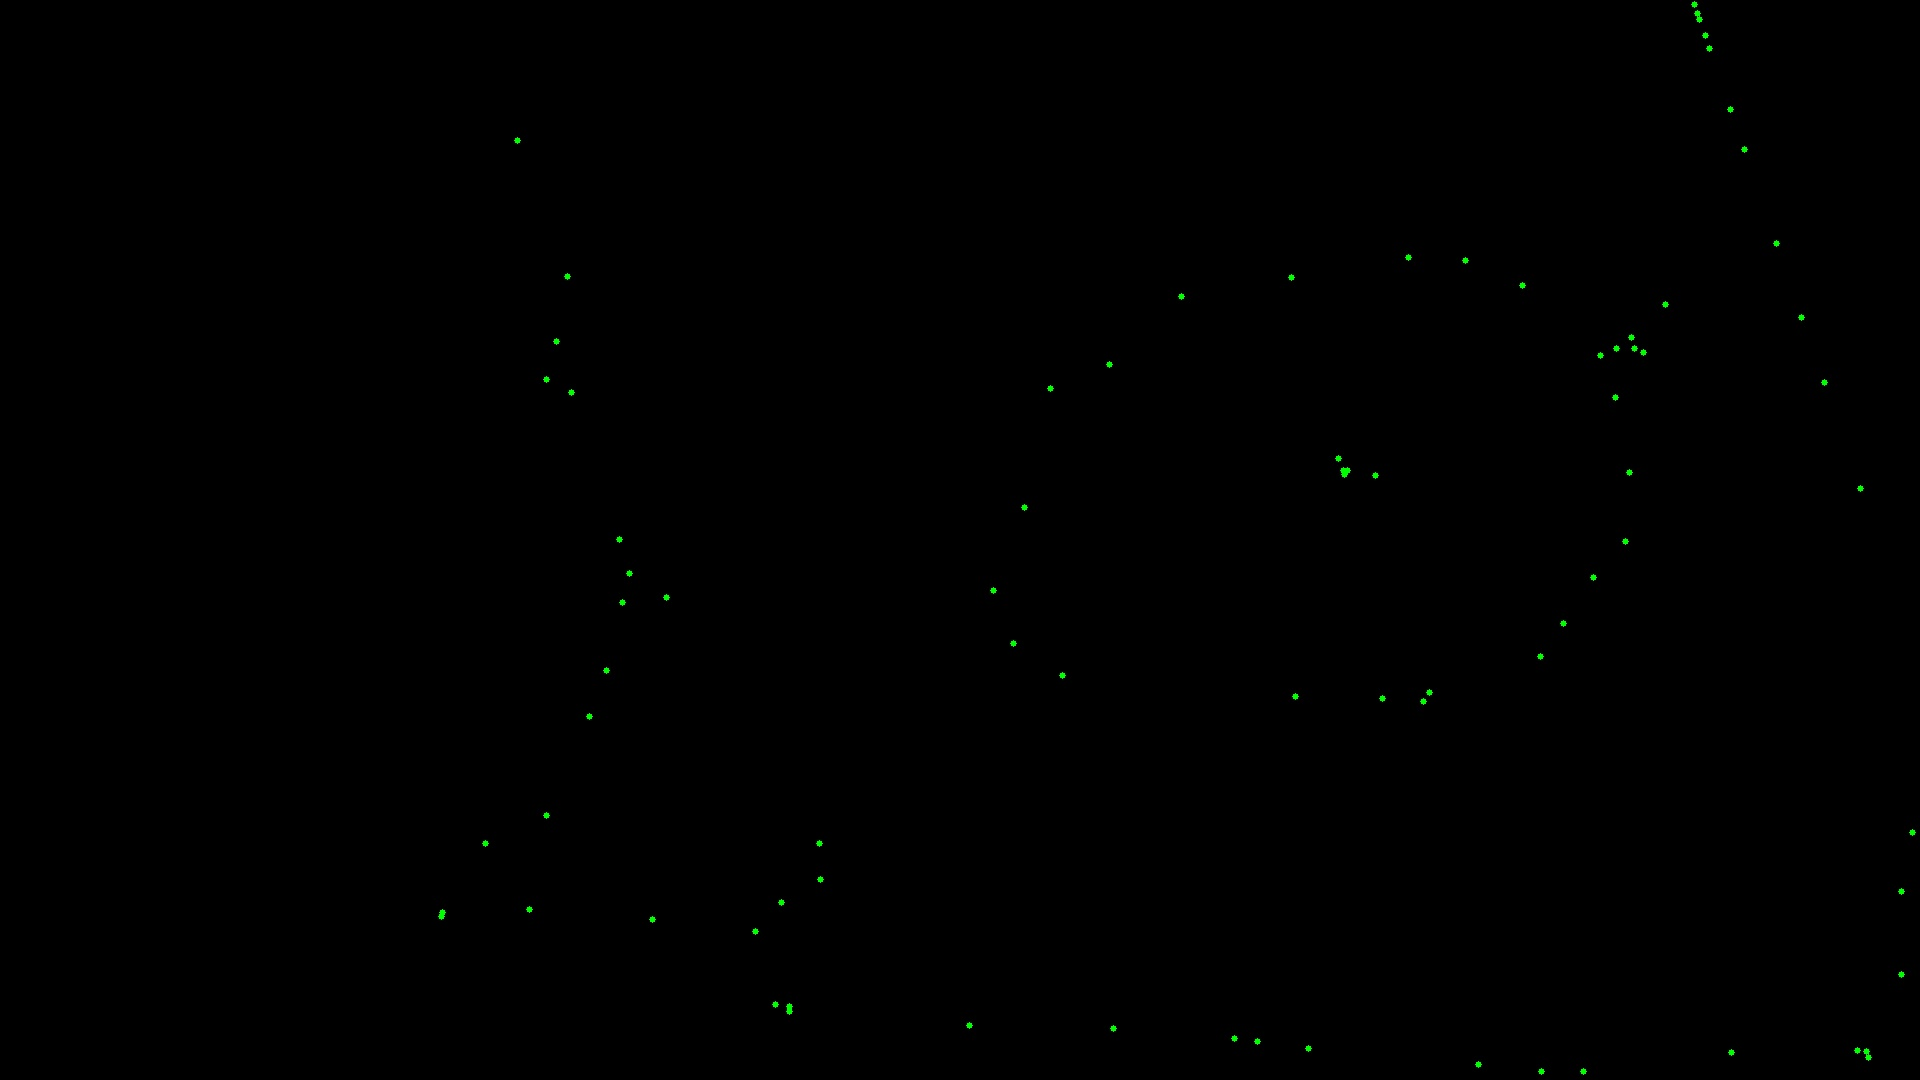
\includegraphics[width=6 cm]{result6_board.jpg}
	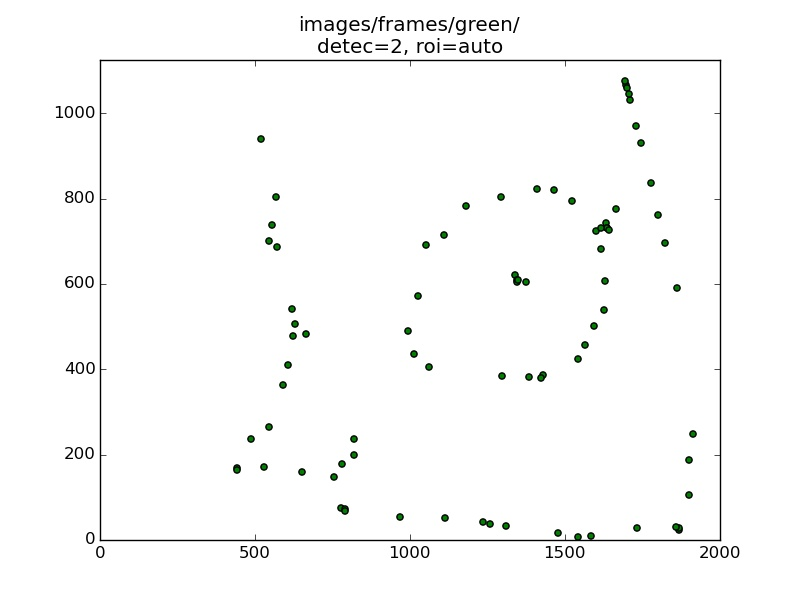
\includegraphics[width=6 cm]{result6_plot.jpg}
	\caption{Board View (left) and plot view (right) of the detection of the marker for 4 different sessions.}
	\label{fig:res}
    \end{center}
\end{figure}
\end{itemize}
%---------------------------------------------------------------------------------------------%
%\subsection*{Risks}
%\begin{itemize}
%\item The computational power required by processing a synced input from two cameras could be a challenge as mentioned in \cite{martin}.
%\item The frame rate of the cameras has to be taking into account. A low frame rate means that fast moves will be hard to identify, while a high frame rate implies more frames to process.
%\item Illumination condition may inquire in difficulties when detecting the marker. Even when we have installed a halogen light source, we still could face some problems due to interference from other sources.
%\item Computational speed. We may suffer from a delay when drawing and projecting the detected strokes in the board due to the amount of processing we need in order produce the output. This could be seen if we make strokes in the board and the drawing is shown with some seconds (hopefully seconds) of delay.
%\item Depending on the frame rate of the cameras, we could suffer from systematic errors. This would imply that the accuracy of the drawing won't that the accuracy of the drawing won't be high, affected by the synchronization procedure mentioned before.
%\item The projected image has already a distortion due to the video-projector position. This could affect the measurement of the accuracy of the system.
%\end{itemize}

%---------------------------------------------------------------------------------------------%
\section[Evaluation Strategy]{Evaluation Strategy\footnote{NLA}}
We proposed to evaluate the system by two criteria:
\begin{itemize}
\item Accuracy: we project a set of raw shapes into the screen as a guideline for testing. Then we capture a session where the shape contours are followed with the marker for comparison between the projected points (output of the system) and the guidelines (ground truth). One drawback of this evaluation strategy is the systematic errors introduced by the human user; e.g., a human can't achieve 100\% accuracy when following the guidelines/contours.
\item Time: we thought of measuring the time the system needed to show the re-projected marker in the board with respect to the time the marker was there. In other words, the delay between input and output of the system (how fast it is and if it works in real time). Sadly, as mentioned before, the system does not work in online mode, therefore, such criteria was abandoned.
\end{itemize}
%--------------------------------------------------------------------------------------------%
\section[Conclusions]{Conclusions}
We offer an approach for designing a virtual board. We sum up some techniques applied to the solution of the problem and we are well aware of must needed improvements. Nevertheless, we can extract some conclusions from the work we developed.


The capture of frames by our system is bad. The frame rate is variable and depends on the availability of RAM the laptop presents. At max we estimate a fps of 10, being this too slow. As a consequence, rapid movement of the marker lead to problems in the detection stage. Sometimes the sphere, which is our object-to-detect was not as sphere; instead, it was a blurry cylinder result of a slow frame rate and a fast motion.


Due to this issue, we failed to implement the Hough Circle Transformation for detection circles in the frames. When the "sphericity" of the markers was lost, the transformation was not able to find circles. For this reason a contour detection was implemented, which rely in color and background. Relying in color is a risk decision to take, given that lighting condition were not completely controllable; this meant that color thresholding does not applies for the same color sphere when the light change drastically. Such phenomena make our system high sensible against light.\footnote{AOS}


Contour as a detection method offers no high robustness. Due to the change in size of the sphere (relatively to the closeness of the marker to the cameras), relying on area as a descriptor is not a good idea. That was experienced many times, when some other contours were given the tag of "marker" just because their area was bigger; in the same manner, when the marker left the scene, some regions were big enough to be tagged as markers (false positives), producing errors in the output.


Calibration was needed and not implemented. Although we obtain the intrinsic parameter of the cameras, we were not able to combine the multiple-view geometry to reconstruct the 3D coordinates of the marker by correspondence. The homography approach offers a easy alternative to achieve this, but not the proper one. Perhaps, rectification of the images using the intrinsics parameter of each camera could lead to better results.


Finally, hardware issues delayed the progress of the project. We were not able to record videos or to access the parameters of the cameras; the second one became an issue when we found out the cameras had an autofocus feature embedded, which we were not able to turn off.\footnote{NLA}


\section*{Annex A: Project division.}
\begin{description}
\item[Argentina] Data capture
\item[Argentina] Marker detection (color).
\item[Nicolas] Marker detection (background segmentation)
\item [Argentina] Color recognition.
\item[Nicolás] Marker pixel coordinates
\item[Nicolás]Position reconstruction
\item[Argentina]Point re-projection

\end{description}
\nocite{*}

\bibliographystyle{unsrt}
\bibliography{Project}


%---------------------------------------------------------------------------------------------%
\end{document}